\secrel{Радиомонтажный инструмент}\secdown

% Пара надфилей, заточной камень на дрель, комплект сверел и несколько листов
% наждачки.
% 
% \subsection{Pro'sKit}
% Отдельного обзора заслуживает инструмент и наборы Pro'sKit
% % \href{http://www.proskit.com/}{ProsKit}
% %  / \href{http://www.proskit.msk.ru/index.html}{ru}.
% 
% \clearpage
% \noindent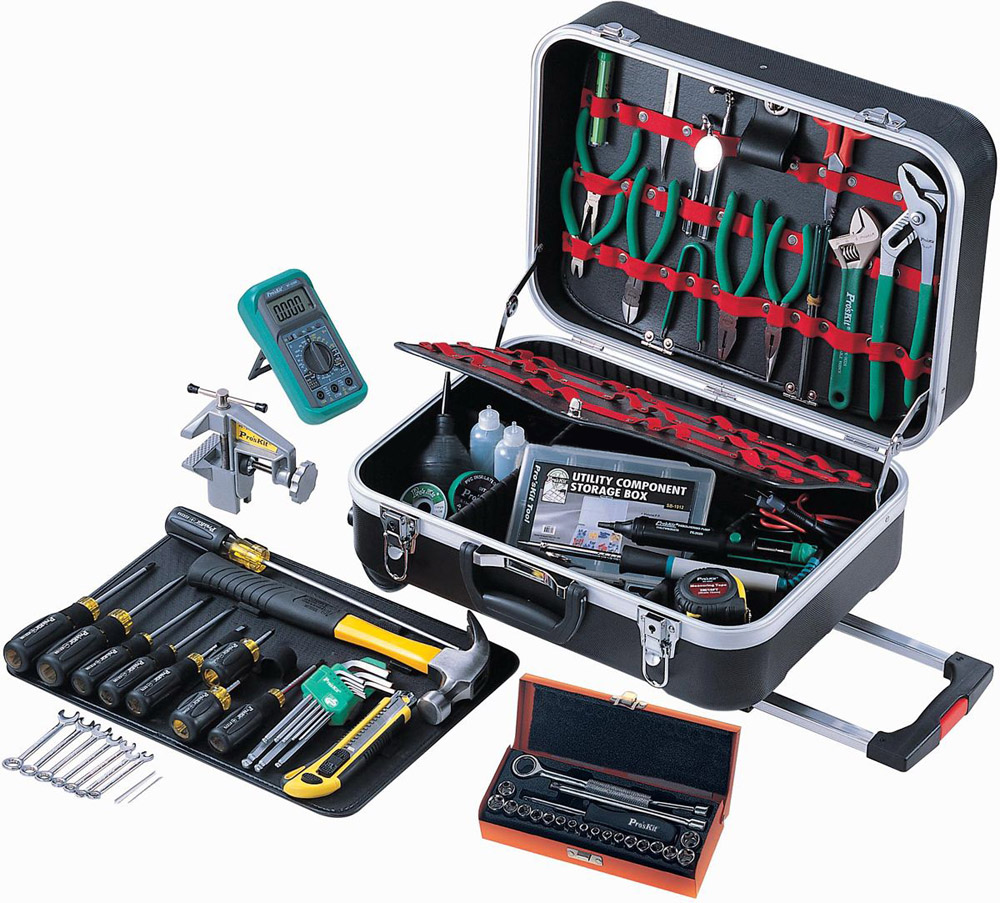
\includegraphics[height=0.95\textheight]{tech/tools/proskit/PK5308BM.jpg}
% 
% \textbf{PK-5308BM универсальный набор инструментов}
% 
% \clearpage
% \noindent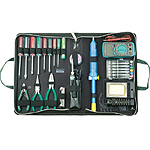
\includegraphics[height=0.95\textheight]{tech/tools/proskit/1PK-616B.jpg}
% 
% \textbf{1PK-616B Набор инструментов для электроники профессиональный}
% 
% \clearpage\label{1PK-813B}
% \noindent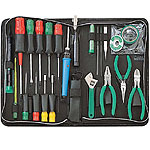
\includegraphics[height=0.95\textheight]{tech/tools/proskit/1PK-813B.jpg}
% 
% \textbf{1PK-813B Набор базовых инструментов для электроники}
% 
% \clearpage
% 
% По личному опыту: в 1PK-813B не хватает
% 
% \begin{itemize}
%   \item мелкого мультиметра, 
%   \item стриппера 1PK-3001E, 
%   \item микрокусачек типа 8PK-30D, 
%   \item канифоли, 
%   \item ножа, 
%   \item настроечную отвертку заменить индикаторной.
% \end{itemize} 
% 
% \clearpage
% \subsubsection{Инструмент до 1000\,В}
% 
% Для электромонтажных работ обязательно приобретите комплект
% высоковольтного инструмента до 1000\,В:
% 
% \begin{tabular}{p{0.45\textwidth} p{0.45\textwidth}}
% \noindent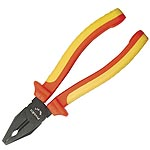
\includegraphics[width=0.45\textwidth]{tech/tools/proskit/PM-911.jpg}
% &
% \noindent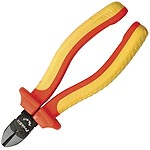
\includegraphics[width=0.35\textwidth]{tech/tools/proskit/PM-917.jpg}
% \\
% 
% \textbf{PM-911 Пассатижи 1\,кВ}
% &
% \textbf{PM-917 Кусачки (бокорезы) 1\,кВ}
% \\
% \end{tabular}
% \clearpage
% 
% \subsubsection{Хранение}
% 
% \begin{tabular}{p{0.45\textwidth} p{0.45\textwidth}}
% \noindent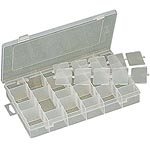
\includegraphics[width=0.45\textwidth]{tech/tools/proskit/103-132D.jpg}
% &
% \noindent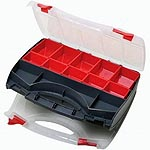
\includegraphics[width=0.45\textwidth]{tech/tools/proskit/SB-3428SB.jpg}
% \\
% \textbf{103-132D Кассетница для деталей и компонентов}
% &
% \textbf{SB-3428SB Портативная кассетница для саморезов и т.п.}
% \\
% \end{tabular}
% \clearpage
% 
% \subsubsection{Радиомонтаж}
% 
% \begin{tabular}{p{0.45\textwidth} p{0.45\textwidth}}
% \noindent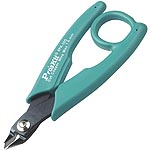
\includegraphics[width=0.45\textwidth]{tech/tools/proskit/8PK-30D.jpg}
% &
% \noindent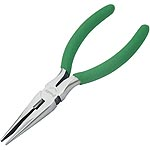
\includegraphics[width=0.45\textwidth]{tech/tools/proskit/1PK-709.jpg}
% \\
% \textbf{8PK-30D Кусачки миниатюрные}
% &
% \textbf{1PK-709 Длинногубцы-кусачки}
% \\
% \end{tabular}
% \clearpage
% 
% \begin{tabular}{p{0.45\textwidth} p{0.45\textwidth}}
% \noindent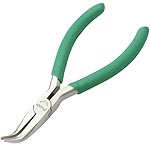
\includegraphics[width=0.45\textwidth]{tech/tools/proskit/1PK-055S.jpg}
% &
% \noindent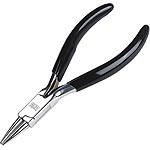
\includegraphics[width=0.45\textwidth]{tech/tools/proskit/1PK-29.jpg}
% \\
% \textbf{1PK-055S Длинногубцы изогнутые}
% &
% \textbf{1PK-29 Круглогубцы}
% \\
% \end{tabular}
% \clearpage
% 
% \begin{tabular}{p{0.45\textwidth} p{0.45\textwidth}}
% \noindent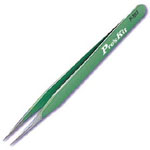
\includegraphics[width=0.45\textwidth]{tech/tools/proskit/1PK-101T.jpg}
% &
% \noindent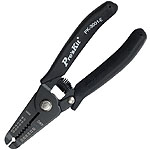
\includegraphics[width=0.45\textwidth]{tech/tools/proskit/1PK-3001E.jpg}
% \\
% \textbf{1PK-101T Пинцет прямой}
% &
% \textbf{1PK-3001E Клещи для зачистки проводов прецизионные (стриппер)}
% \\
% \end{tabular}
% \clearpage
% 
% \begin{tabular}{p{0.45\textwidth} p{0.45\textwidth}}
% \noindent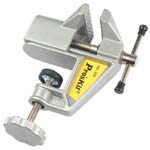
\includegraphics[width=0.45\textwidth]{tech/tools/proskit/PD-374.jpg}
% &\\
% \textbf{PD-374 Тиски на струбцине}
% &\\
% \end{tabular}
% \clearpage
% 
% \subsubsection{Прочие}
% 
% Попалась интересная недорогая отвертка: aиксация четкая, исполнение очень
% неплохое, позволяет добраться до узких мест. Из минусов: ручка похоже не
% цельнометаллическая, при изломе есть риск распороть руку.
% 
% \bigskip
% \noindent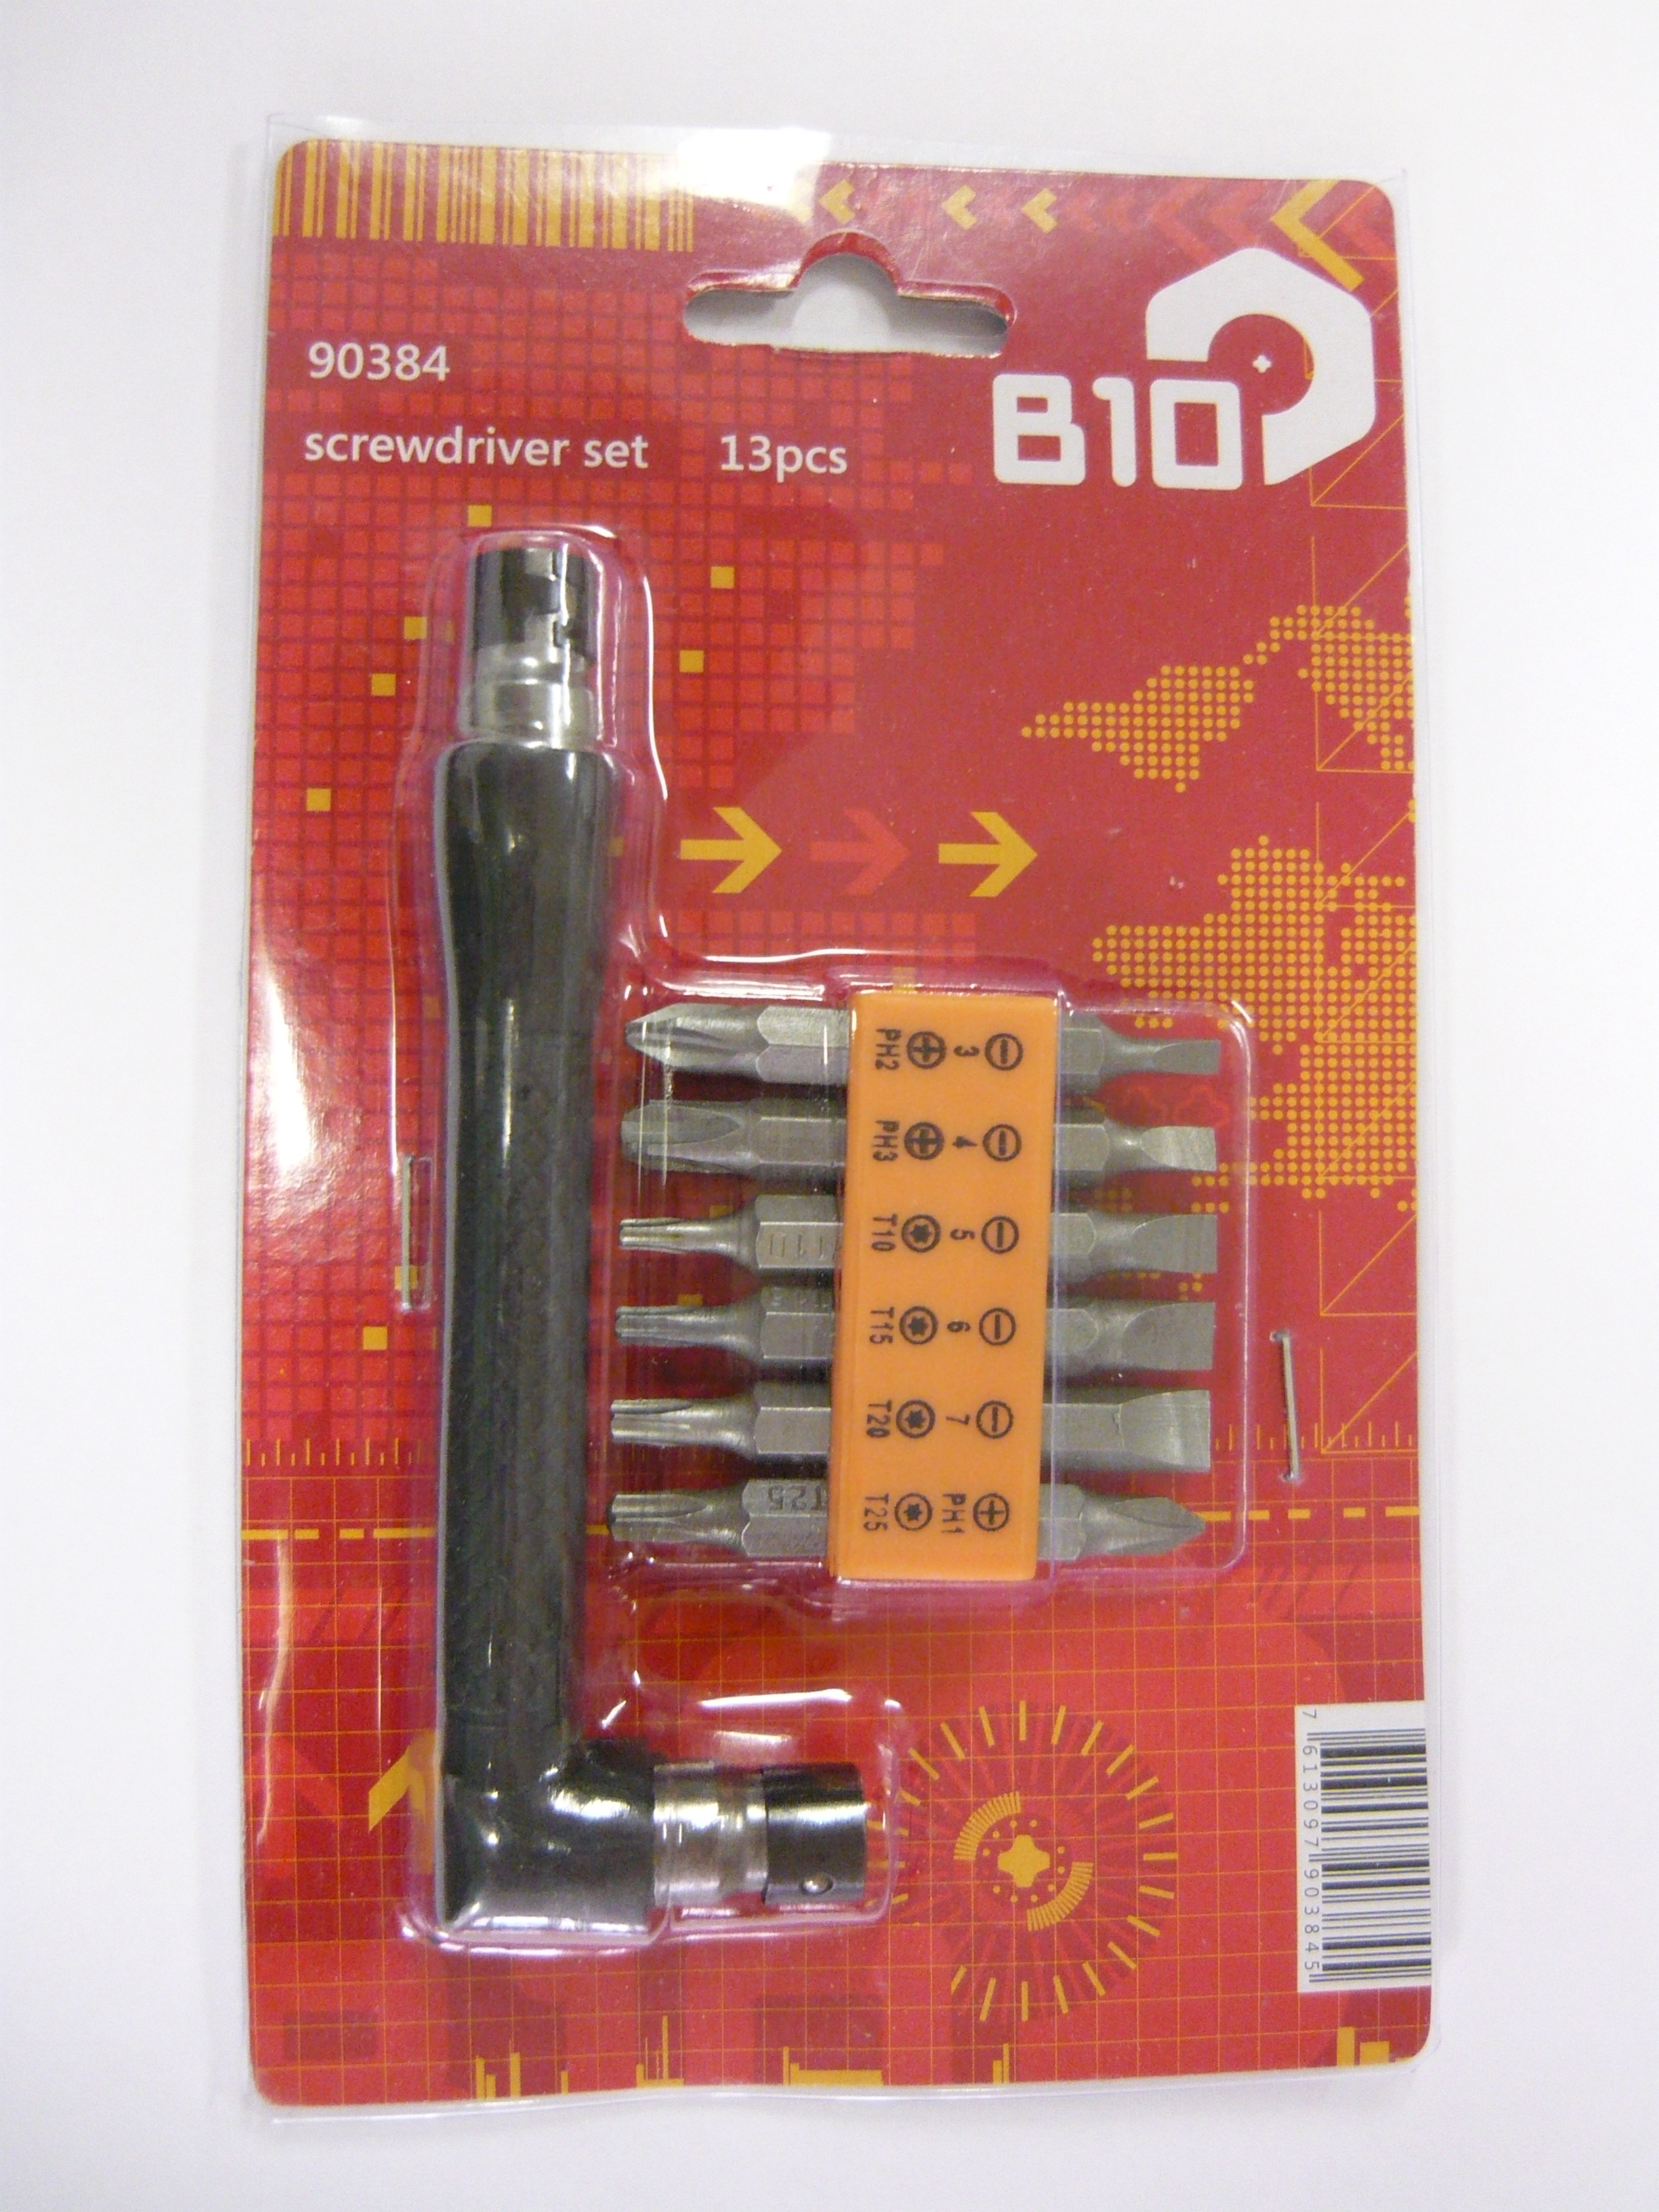
\includegraphics[width=0.4\textwidth]{tech/tools/P1020966.jpg}
% \noindent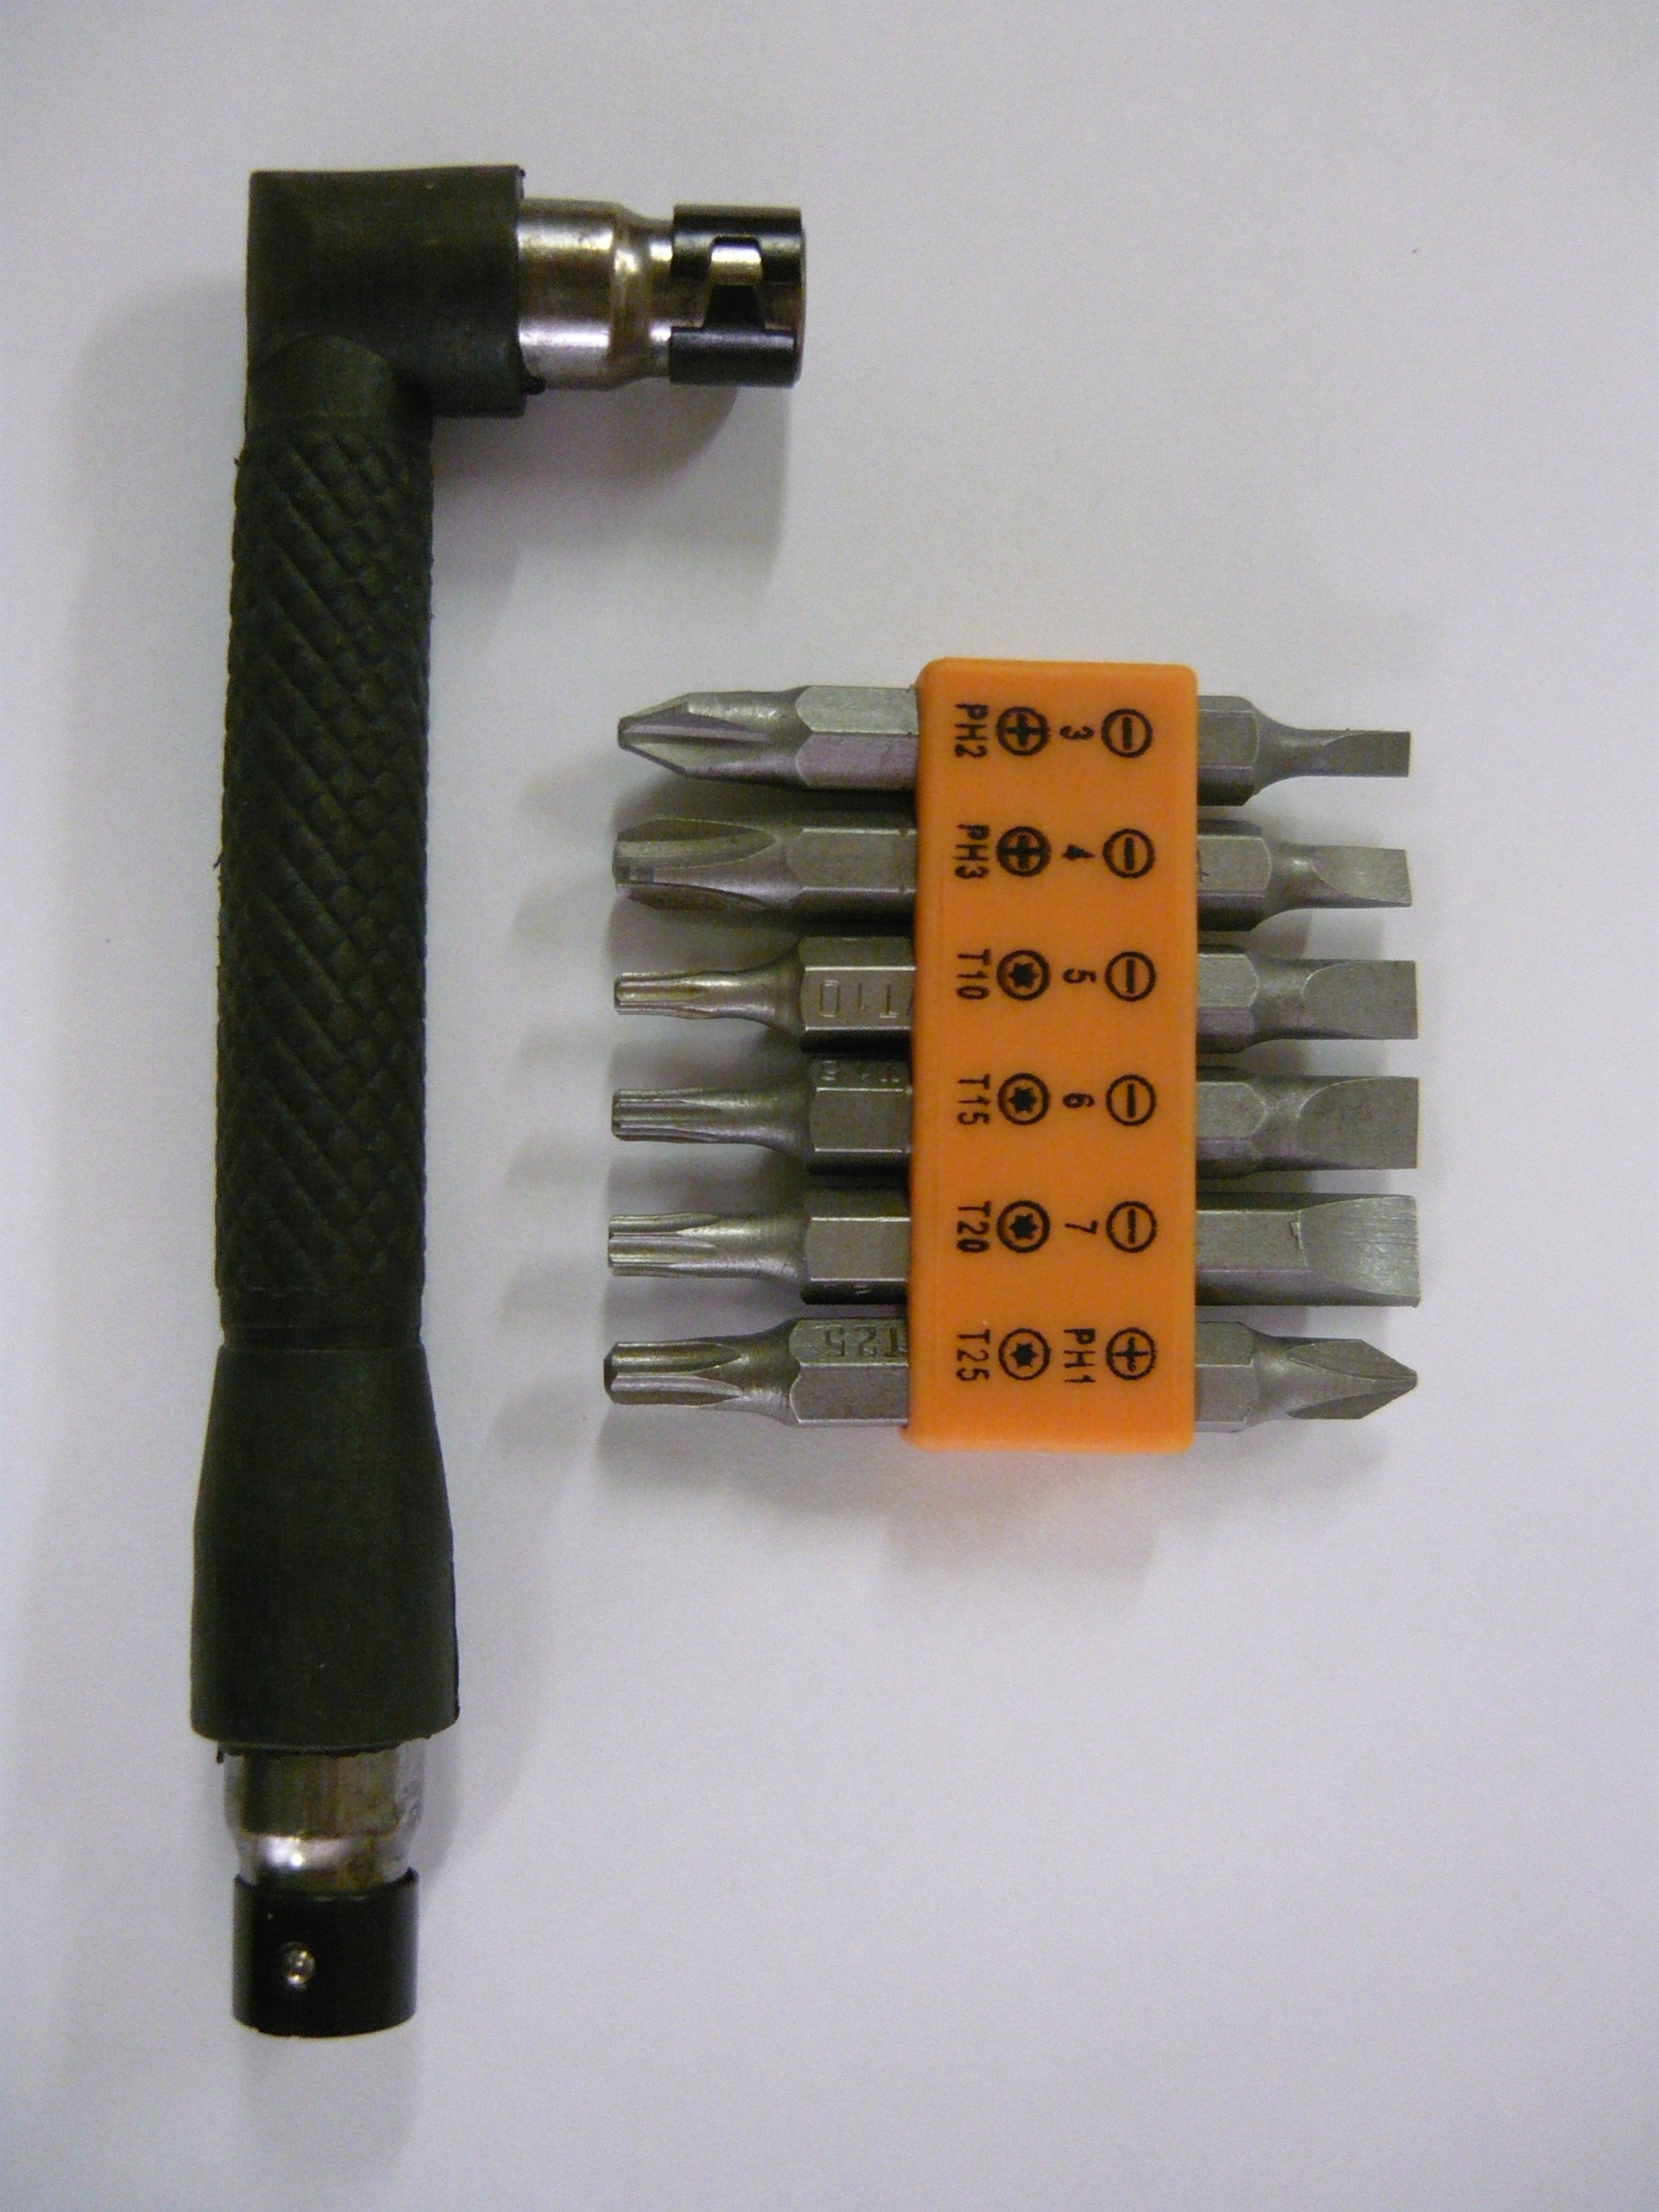
\includegraphics[width=0.4\textwidth]{tech/tools/P1020967.jpg}
% \clearpage

\secup

